% Metódy inžinierskej práce

\documentclass[12pt,twoside,slovak,a4paper]{article}
\usepackage[
  top=1in,
  bottom=1in,
  left=1.5in,
  right=1.5in
]{geometry}

\usepackage[slovak]{babel}
\usepackage[T1]{fontenc}
\usepackage[utf8]{inputenc}
\usepackage{lmodern} % moderný font
\usepackage{microtype} % zlepšenie sadzby
\usepackage{graphicx}
\usepackage{url}
\usepackage{hyperref}
\usepackage{titlesec} % prispôsobenie nadpisov
\usepackage{booktabs} % pre peknejšie tabuľky
\usepackage{cleveref} % inteligentné referencie
\usepackage{indentfirst} % zarezávanie prvého riadku po nadpise
\usepackage{float} % Ku tabulke


\title{Ako algoritmy sociálnych médií získavajú informácie 
z používateľov a následne ich využívajú vo svoj 
prospech}

\author{David Vach\\
	{\small Slovenská technická univerzita v Bratislave}\\
	{\small Fakulta informatiky a informačných technológií}\\
	{\small \texttt{xvachd@stuba.sk}}\\
	{\small Vedenie: Mirwais Ahmadzai}
}

\date{\small 16. december 2023} 

% Definície štýlov nadpisov
\titleformat{\section}
  {\normalfont\Large\bfseries}
  {\thesection}{2em}{}

\titleformat{\subsection}
  {\normalfont\large\bfseries}
  {\thesubsection}{1em}{}

% Vlastné definície pre abstract a kľúčové slová
\newcommand{\keywords}[1]{
  \small	
  \textbf{\textit{Kľúčové slová---}} #1
}

\begin{document}

\maketitle

\begin{abstract}
Tento článok sa bude venovať podrobnej analýze získavaniu informácii používateľov sociálnych médií pomocou algoritmov. Práca bude pozostávať z toho ako sa tieto algoritmy snažia získať čo najviac informácií z používateľov, ktoré následne môžu využiť na rôzne marketingové ciele. Jadro tohto článku sa sústreďuje na algoritmy a ich efektivite v udržiavaní pozornosti používateľov na základe získaných dát a následné zobrazovanie špecifického obsahu za účelom získať čo najviac presnejších dát a následné vymazávanie nepotrebných dát. Ďalšia časť tejto práce ukazuje rôzne spôsoby zneužívania týchto dát vo svoj prospech z dlhodobého hľadiska a ako tieto algoritmy vedia pomocou získaných dát určiť s veľkou pravdepodobnosťou osobnosť používateľa a iné citlivé informácie. Záver práce tvoria dôvody prečo by sme si mali tieto súkromné dáta chrániť a aké spôsoby sa na to využívajú.
\end{abstract}

\keywords{sociálne médiá, zber dát, ochrana súkromia, algoritmy, marketing}

\newpage
\section{Úvod}

V úvode dnešnej digitálnej éry predstavujú sociálne médiá viac než len platformy na zdieľanie osobných príbehov a fotografií. Sú to sofistikované ekosystémy využívajúce algoritmy, ktoré transformujú spôsob, akým komunikujeme, angažujeme sa a dokonca ako sa rozhodujeme. Algoritmy sociálnych médií sú navrhnuté tak, aby boli nenápadnými, no mocnými kustódmi našej online pozornosti. Vychádzajú zo záveru, že každá interakcia na platforme - lajk, zdieľanie, komentár, dokonca aj dĺžka zdržania sa pri príspevku - je cenným údajom, ktorý odhaľuje náš vkus, preferencie a správanie. Tieto údaje sú potom analyzované a transformované na mieru, ktorá nás drží zapojených – a často prilepených – na naše obrazovky dlhšie než sme plánovali.
No táto personalizácia má aj svoju cenu. Algoritmy sociálnych médií sú takisto navrhnuté na podporu obchodných modelov ich prevádzkovateľov, čo znamená, že informácie získané z používateľských interakcií sú často využívané na cieľovú reklamu a obsahové odporúčania, ktoré podporujú angažovanosť a zisky. V tomto procese sú používatelia niekedy nevedomky manipulovaní k tomu, aby konzumovali obsah a produkty, ktoré možno nepotrebujú alebo dokonca nechcú. Tento úvod bude skúmať, ako algoritmy sociálnych médií zbierajú a využívajú používateľské informácie a aké sú implikácie tohto procesu na súkromie, spoločenské správanie a dokonca na demokraciu. V tejto sekcii by som sa chcel venovať tomu, čo mňa motivovalo k tejto téme. Myslím si, že rýchlym rozširovaním online sociálnych médií si veľa ľudí vyberá, aby svoje názory na určité témy vyjadrovali práve v týchto sieťach, vrátane komentárov k produktom a službám. V období veľkých dát poskytuje nárast používateľmi vytvorených komentárov k produktom či iným veciam. Preto na sociálnych sieťach vznikajú rôzne príležitosti pre firmy na získanie cenných obchodných informácií pre lepšie rozhodovanie. Keďže komentáre zverejnené na Facebooku alebo Instagrame sa veľmi často odrážajú na individuálne postoje ľudí k špecifickým produktom alebo službám, môžu byť zneužité na riešenie obchodných problémov rôznych firiem. 

Môžme si všimnúť, že podrobná analýza sentimentu používateľov na online sociálnych médiách môže poskytovať dôležité informácie (dáta) pre obchodné rozhodovanie. Preto v navrhovanom rámci analýzy sentimentu delíme jednotlivcov (aktérov) sociálnych sietí do troch skupín na základe ich odlišných orientácií názorov na produkt, a to: 
(a) skupina P obsahuje aktérov, ktorí majú k produktu pozitívny názor
(b) skupina N zahŕňa aktérov, ktorí produkt nemajú radi a prejavujú negatívnu orientáciu názorov
(c) skupina U obsahuje aktérov, ktorí majú k produktu neutrálny (ambivalentný) postoj.
\cite{7809906}

\section{Súvisiaca práca} 
\cite{7809906}
\cite{7087040}

%Túto sekciu by som chcel venovať hlavne zdrojom a citáciam, ktoré sa budú v tomto článku nachádzať. Primárne ma k tejto téme priviedol tento článok, na ktorý sa budem veľmi často obracat, pretože podobrobne opisuje danú problematiku z rôznych uhlov pohľadu.\cite{7809906} 
%
%Ďalej použité zdroje:
%
%Analysis of Marketplace Social Media User Engagement by Topic\cite{10057722}
%
%Sentiment analysis for the news data based on the social media\cite{8250692}
%
%A Feature Selection Algorithm Based on Pairwise Constraints for Linked Social Media 
%Data\cite{8575882}
%
%Research on Social Media Feature Learning Algorithm Based on Deep Neural Network\cite{9719080}
%
%Empirical Analysis of User Factors that Affect the User Interface Design in Mobile 
%Applications\cite{9325452}
%
%Efficient regression algorithms for classification of social media data\cite{7087040}
%
%Sentiment analysis for the news data based on the social media\cite{8250692}
%
%Topic modeling for social media content: A practical approach\cite{7783248}


\section{Ako tieto algoritmy fungujú}
Algoritmy sociálnych médií sú navrhnuté tak, aby efektívne zbierali a analyzovali údaje generované užívateľmi pri ich interakciách online. Ich schopnosť poskytovať personalizovaný obsah je založená na dômyselnom sledovaní a vyhodnocovaní činností používateľov. Keď používateľ lajkuje príspevok, komentuje video alebo strávi určitý čas čítaním článku, tieto akcie sú zaznamenané a stávajú sa časťou veľkého údajového modelu, ktorý tento algoritmus používa na pochopenie a predvídanie preferencií používateľa.

Na základe textu, obrázkov a videí, ktoré používatelia zdieľajú alebo komentujú, algoritmy využívajú pokročilé metódy ako spracovanie prirodzeného jazyka a rozpoznávanie obrazu na to, aby lepšie porozumeli obsahu, ktorý používatelia preferujú. Algoritmy zároveň skúmajú vzťahy a interakcie medzi používateľmi, aby zistili, aké sociálne siete sú pre nich najdôležitejšie a ako sa tie môžu prepojiť s ich obsahovými preferenciami.

Na základe získaných dát tieto algoritmy vytvoria obsah, ktorý sa používateľom zobrazuje vo feedoch, aby bol čo najrelevantnejší a najzaujímavejší. Tento personalizovaný prístup sa nezameriava len na zvýšenie užívateľskej spokojnosti a zapojenia, ale je tiež základom pre efektívnu cieľovú reklamu, kde sú reklamy prispôsobené konkrétnym záujmom a správaniu používateľov.

Súčasťou procesu je aj predpovedanie správania. Algoritmy sociálnych médií sa pokúšajú predvídať, čo by mohlo používateľov zaujímať v budúcnosti, a prispôsobujú svoje stratégie, aby bol obsah, ktorý zobrazujú, vždy krok vpred. Vďaka neustálej spätnej väzbe a iterácii sa algoritmy neustále učia a zdokonaľujú, aby boli ešte lepšie v predvídavaní a napĺňaní očakávaní užívateľov.


Názorný príklad pre Facebook:

\begin{figure}[h]
    \centering
    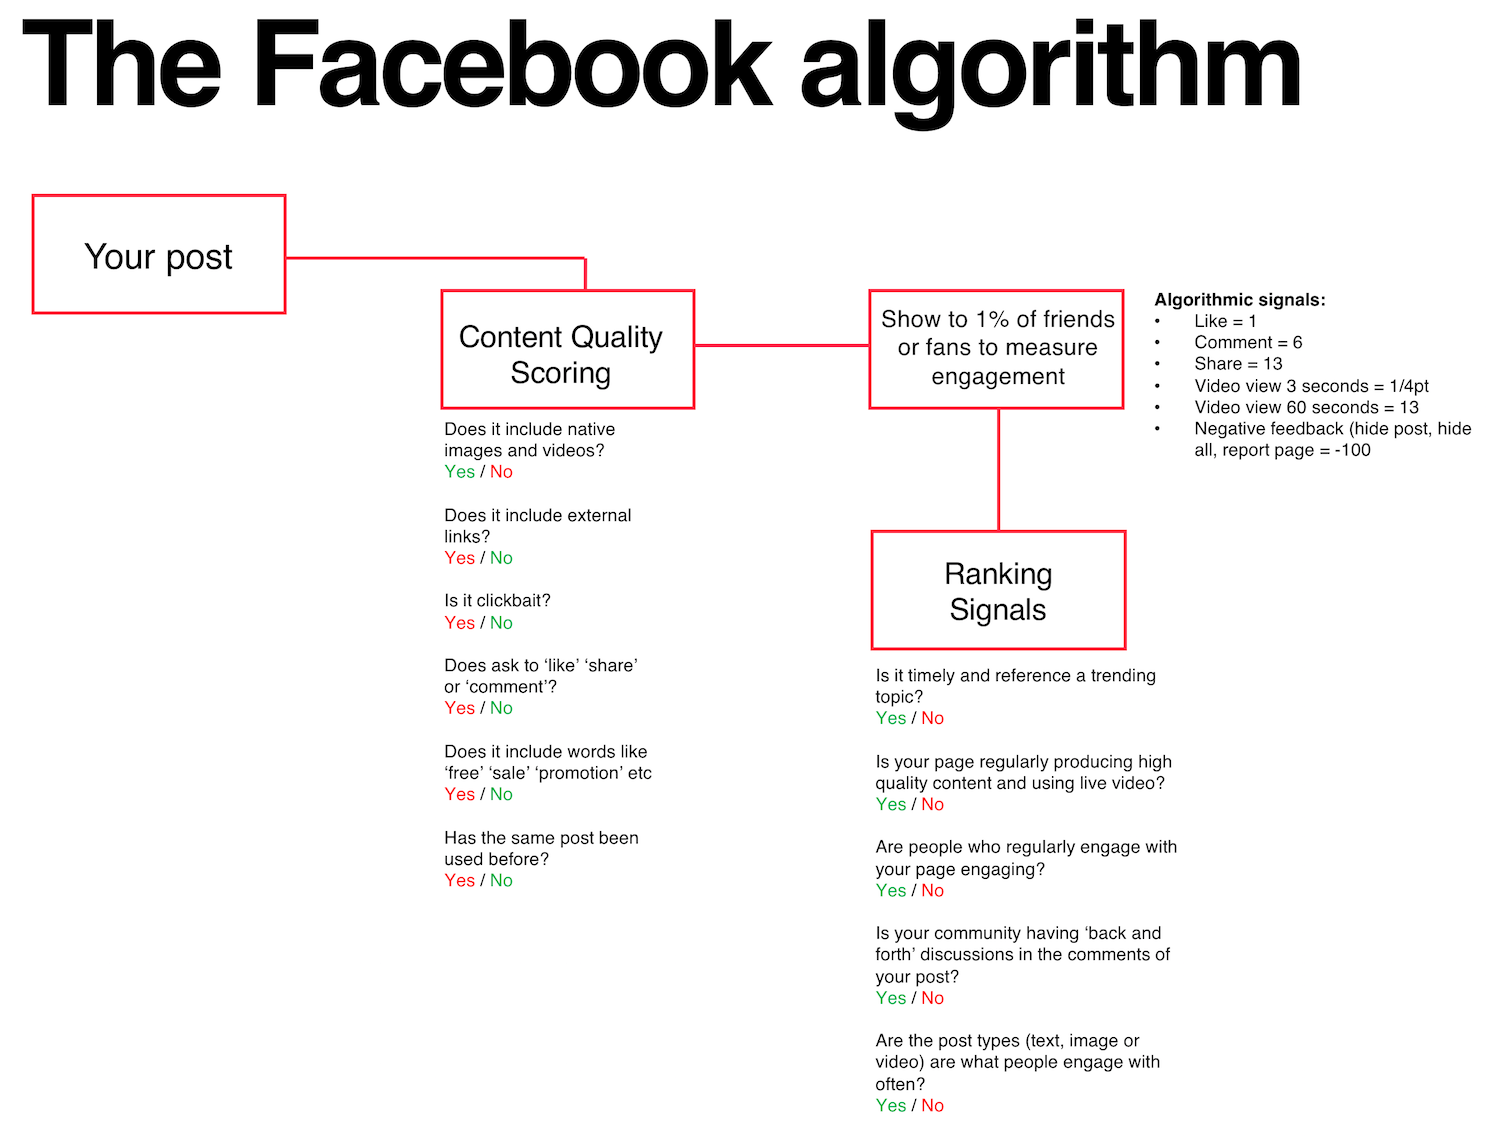
\includegraphics[scale=0.6]{dd3ba30631ea2b442e37f156fe8b0189.PNG} 
     \cite{kontostathis2006}\caption{Truncation of SVD for LSI.}
    \label{fig:truncation}
\end{figure}


Výsledkom je, že algoritmy sociálnych médií tvoria dynamický a neustále sa vyvíjajúci systém, ktorý je mimoriadne citlivý na potreby a chovanie používateľov, a to všetko v úsilí udržať ich zapojenie a poskytnúť im maximálne prispôsobený zážitok. Ekonomický model sociálnych sietí, založený predovšetkým na reklamných príjmoch, je priamo ovplyvnený úspešnosťou týchto algoritmov v predpovedaní a ovplyvňovaní používateľského správania.





\section{Metodológia}

V rámci tejto štúdie sme sa zameriavali na analýzu algoritmov sociálnych médií a ich vplyvu na správanie používateľov. Metodológia našej práce zahŕňala niekoľko kľúčových krokov. Začali sme výberom relevantných dátových sád zo sociálnych médií, pričom sme sa zamerali na obdobie posledných dvoch rokov. Tieto dáta zahŕňali používateľské interakcie, ako sú lajky, komentáre a zdieľanie obsahu. Následne sme analyzovali špecifické algoritmy používané týmito platformami, vrátane NaiveBayes a Adaboost, pričom sme hodnotili ich efektivitu v personalizácii obsahu a vplyve na používateľské správanie. Použili sme techniky spracovania prirodzeného jazyka a analýzy sentimentu na spracovanie týchto dát. Počas celého procesu sme si boli vedomí etických zvážení spojených so zberom a analýzou používateľských dát. Na vyhodnotenie účinnosti rôznych algoritmov sme použili špecifické metriky, ako sú miera zapojenia a čas strávený používateľmi na platforme. Táto metodológia nám umožnila poskytnúť hĺbkový pohľad na to, ako algoritmy sociálnych médií ovplyvňujú používateľské správanie a súkromie.


\section{Analýza}
Porovnavane algoritmy:

\begin{table}[h]
\centering
\begin{tabular}{|l|p{4cm}|p{4cm}|p{3cm}|}
\hline
\textbf{Algorithm} & \textbf{Advantages} & \textbf{Disadvantages} & \textbf{Best Use Case} \\
\hline
Adaboost & Improves weak models, adaptable & Sensitive to noise, prone to overfitting & Classification with 'difficult' cases \\
\hline
NaiveBayes & Simple, fast, effective for text data & Assumes independence of features, can be less accurate & Text classification, spam filtering \\
\hline
GBM & High accuracy, effective for complex patterns & Prone to overfitting, computationally intensive & Classification and regression with complex patterns \\
\hline
Random Forest & Resistant to overfitting, effective for large datasets & Less interpretable, computationally intensive & Classification and regression, large datasets \\
\hline
\end{tabular}
\caption{Comparison of Machine Learning Algorithms}
\label{table:algorithm_comparison}
\end{table}






\subsection{NaiveBayes\cite{7809906}}

\subsection{Adaboost\cite{7087040}}

\subsection{Random Forest\cite{9952138}}

\subsection{Gradient Boosting Machines (GBM)\cite{9952143}}
















\section{Výsledok}


\section{Záver} 

PREDBEZNY ZAVER:

V našej štúdii sme skúmali, ako algoritmy sociálnych médií získavajú a využívajú informácie od používateľov. Naše zistenia ukazujú, že tieto algoritmy hrajú kľúčovú úlohu v personalizácii používateľského obsahu a v ovplyvňovaní správania používateľov. Avšak spolu s týmto prispôsobením prichádza aj zvýšené riziko zneužitia používateľských údajov a narušenia súkromia. Preto je nevyhnutné, aby sa pri vývoji a implementácii týchto algoritmov kládol dôraz na etické zváženia a ochranu súkromia. Naše výskumy naznačujú potrebu väčšej transparentnosti a regulácie v oblasti algoritmov sociálnych médií, aby sa zaistila ochrana používateľov a ich údajov.




\section{Reakcia na prednášky}

\subsection{Kreatívne písanie (Prednáška 8)}

Kreatívne písanie je umenie, ktoré umožňuje autorom vyjadriť svoje myšlienky, emócie a predstavy prostredníctvom slov. Je to proces, ktorý spočíva v tvorbe originálnych textov, či už ide o poéziu, prózu, drámu alebo iné literárne formy. Pri kreatívnom písaní je dôležitá nielen schopnosť gramaticky správneho a zrozumiteľného vyjadrovania, ale predovšetkým originalita a kreativita. Autor by mal byť schopný preniesť čitateľa do svojho sveta, ukázať mu nové perspektívy a vyvolať v ňom emócie.

Kľúčom k úspechu v kreatívnom písaní je pravidelná prax a ochota experimentovať so slovami a štýlom. Dobrý autor by mal byť otvorený novým nápadom a neprestajne rozvíjať svoje písacie zručnosti. Kreatívne písanie nie je len o výroku umeleckých diel, ale aj o sebavyjadrení a osobnom rozvoji. Táto forma písania môže byť terapeutická a umožňuje autorom vyrovnať sa s osobnými záležitosťami alebo spracovať svoje myšlienky a pocity. Preto je dôležité vytvárať prostredie, kde sa autori cítia inšpirovaní a majú priestor na kreativitu.

\subsection{Plagiátorstvo (Prednáška 9)}
Plagiátorstvo je téma, o ktorej by mal byť každý tvorca článku, eseje, prezentácie alebo autor akéhokoľvek verejného prejavu oboznámený. Dá sa to nazvať krádežou, ale niekedy sa môže človek dopustiť neúmyselnému plagiátorstvu. Spôsob, akým sa mu vyhnúť je jednoduchý, a to odkazovať sa na použité zdroje.

\subsection{Technológia a ľudia: Scrum. doc. Valentino Vranić (Prednáška 11)}
Niaky text pojdem na prednasku


%POZNAMKA K TEJTO SEKCII
%1.
% It is not recommended to include the title of the article in
%the related work section. Instead, provide a brief summary of %the main
%focus of the article in one or two sentences.


%2. Student contribution and research methodology are missing in the
%article.
%
%3. The first lengthy paragraph in the introduction section lacks
%professional structure; consider breaking it down into sub-paragraphs.
%
%4. The first paragraph in the introduction lacks citations, making it
%unclear whether the ideas presented are the student's or from other
%sources.
%
%5. Ensure that reference numbers are in ascending order, and correct the
%"?" mark in some citations, such as the one in the diagram



%LITERATURA
\bibliographystyle{abbrv}
\bibliography{bibtex.bib}

%KONIEC DOKUMENTU
\end{document}